\section{Aerodynamic database}
In this section, it is explained how the aerodynamic database was obtained to study the effect of varying the vertical tail surface area. Assumptions are re-called to put the focus only on relaxed lateral stability.

\subsection{Reference Aircraft}
The method developed up to now is generic and could be used with any aircraft given the corresponding aerodynamic characteristics. To study the differences between a traditional configuration and a DEP aircraft, a baseline aircraft representing the class of aircraft most probable for electric propulsion and distributed propulsion has to be selected. Commuters aircraft are often cited as the next big step in developing electric airplanes since most of their mission are within the limits of electric propulsion in terms of endurance \cite{MisconceptionMoore} \cite{StucklMethodsDesignElectriProp}. These aircrafts usually are equipped with turboprop engine and fly at subsonic velocity. A good representative of this class of aircraft is the ATR72 which details are reported in table~\ref{tab:nominalset}.

\begin{table}[hbt!]
	\caption{\label{tab:nominalset} ATR 72 general details \cite{ATRFAAtypecertificate}, \cite{JanesAircraft}}
	\centering
	\begin{tabular}{l|c}
		Variables & Value\\
		\hline
		Wingspan & 27 m\\
		Wing surface area & 61 m$^2$\\ 
		VT surface area & $12$ $\textrm{m}^2$\\
		Engine level arm & 4.1 m\\
		Masse & 21500 Kg\\
		Total available power & 4 000 KW\\
		Stall velocity $V_s$ & 56 m/s\\
	\end{tabular}
\end{table}

So far, special care was given to keep the analysis as generic as possible to be able to compare flight qualities of different aircraft configurations. Following the same philosophy it is assumed no change in the geometry, mass or power available of the reference ATR72 between the baseline configuration and the electric propelled one.

The only feature allowed to change is the vertical tail which will be reduced so as to obtain relaxed lateral stability or a lightly unstable aircraft. Consequently, we will analyse a weakly unconventional aircraft configuration.

\subsection{Building the Aerodynamic Database}
For unconventional configurations, it is necessary to carefully select the method with which one can establish the aerodynamic database. As Chudoba explains in \cite{ChudobaUnconventionalConf}, the means of calculating aerodynamic characteristics can be organized in three categories summurised in Table~\ref{tab:aeroAnalysis}.
\begin{table}[hbt!]
	\caption{\label{tab:aeroAnalysis} Methods for Aerodynamic Analysis \cite{Chudoba_generic_method}}
	\centering
	\begin{tabular}{l|c}
		Category & Example of methods\\
		\hline
		Analytical & Lifting Line, Swept Wing Theory, ...\\
		Empirical, semi-empirical & DATCOM, ESDU, ...\\ 
		Numerical & Vortex Lattice Method, Panel Method, CFD, ...\\
	\end{tabular}
\end{table}

Both analytical and empirical/semi-empirical methods are built on experiences and analysis of conventional configurations. Therefore there can hardly be concidered as generic methods. Numerical methods offer different level of fidelity allowing to capture the specificity of unconventional design. For preliminary designs, VLM or Panel Method, both linear technics, are often prefered over CFD for their favorable precision relative to computational cost.

Although our configuration is only weakly unconventional, capturing the effect of geometrical changes in VT isn't something that analytical of empirical/semi-empirical methods can do because of the important influence of other aircraft components on the flow impacting the VT. This has been demonstrated by Nicolosi in \cite{NicolosiInvestigationVertical}, where his research team investigated the differences obtained between DATCOM, ESDU estimation technics and CFD methods complemented with wind tunnel experiments.

The main contributors to flow perturbation impacting the VT are the fuselage and the horizontal tail which are acting as end plates, reducing the downwash at the root and tip of the vertical tail. 

Using numerous CFD simulations complemented with wind tunnel test on a generic commuter aircraft model, Nicolosi and his research team could establish a new semi-empirical method called VeDSC. This method focuses on predicting the VT efficiency as a function of VT geometry and aircraft components. The main assumption is the fact that contribution of each components of the aircraft on lateral coefficients; $C_{Y}$, $C_{p}$, $C_{r}$ $\equiv C_{\textrm{lat}}$, can be decoupled in the following way:
\begin{eqnarray}
C_{\textrm{lat}_\beta} = C_{\textrm{lat},F_\beta} + C_{\textrm{lat},W_\beta} + C_{\textrm{lat},v_\beta}
\end{eqnarray}
Where it is assumed that the contribution of the VT, $C_{\textrm{lat},v_\beta}$ is influenced by the fuselage, wing and horizontal tail but does not influence the other coefficients $C_{lat,F_\beta}$ and $C_{lat,W_\beta}$.
The VeDSC method furnishes a way to estimate the coefficient $C_{\textrm{lat},v_\beta}$ through a reformulation of the VT lift slope coefficient defined as follow:
\begin{equation}
a_v=K_F K_W K_H C_{L,v_\beta}
\end{equation}
Where $C_{L,v_\beta}$ is the lift slope of a swept wing determined using Diederich formula for swept wing \cite{DiederichPlanformParameter}. $K_F$, $K_W$ and $K_H$ are corrective coefficients taking into account respectively the fuselage, wing and horizontal tail effects. The reader is refered to \cite{NicolosiVTDesignReview} and \cite{NicolosiDirectionalStabilityReviewofEmpiricalMethod} for the complete formulation of these parameters.

The VT contribution to lateral coefficients is then calculated using formulas given by Etkin \cite{Etkin}:
\begin{align}
&C_{Y_\beta} = a_v\frac{S_v}{S}\left( 1-\frac{\partial \sigma}{\partial \beta}\right) 
&&C_{l_\beta} =-a_v\frac{S_v z_v}{S b}\left( 1-\frac{\partial \sigma}{\partial \beta}\right) 
&&&C_{n_\beta} = a_v V_v\left( 1-\frac{\partial \sigma}{\partial \beta}\right)\\
&C_{Y_p} = -a_v\frac{S_v}{S}\left(2\frac{z_v}{b}-\frac{\partial \sigma}{\partial \hat{p}}\right) && \qquad &&&C_{n_p}= a_v V_v\left(2\frac{z_v}{b}-\frac{\partial \sigma}{\partial \hat{p}}\right)\\
&C_{Y_r} = a_v\frac{S_v}{S}\left( 2\frac{l_F}{b}+\frac{\partial \sigma}{\partial \hat{r}}\right)  &&C_{l_r} =a_v\frac{S_v z_v}{S b}\left( 2\frac{l_F}{b}+\frac{\partial \sigma}{\partial \hat{r}}\right) &&&C_{n_r} = -a_v V_v\left( 2\frac{l_v}{b}-\frac{\partial \sigma}{\partial \hat{r}}\right)
\end{align}

This semi-empirical methods required hundreds of CFD simulations to explore a wide variety of parameter changes. Variation and validity intervals of some parameters of interest are shown in Table~\ref{tab:VeDSCParam}. The method could be extrapolated to VT of aspect ratio from 0.5 to 4 since the Diederich formula is valid for these values however the correcting terms would be out of interpolation range.



Overall the VeDSC method turns to be an adequate semi-empirical method to be used with our reference aircraft. In addition, having a formula to estimate the VT efficiency instead of running a VLM is an important time saving aspect.

In order to establish our aerodynamic database, we modeled the ATR72 without its VT into VSPaero using publicly available data essentially from \cite{JanesAircraft}. The VLM included in VSPaero is then used to establish the longitudinal coefficients and contribution to the lateral coefficients. The contribution of the fuselage and wing to lateral coefficients has been found to be adequatly estimated by the VLM. It is then complemented with the VeDSC method to quickly and accurately account for the changes in VT geometry. This renders the database extremely agile since we only need to run VLM simulations once.

\begin{figure}[hbt!]
	\centering
	\begin{subfigure}[b]{0.33\textwidth}
		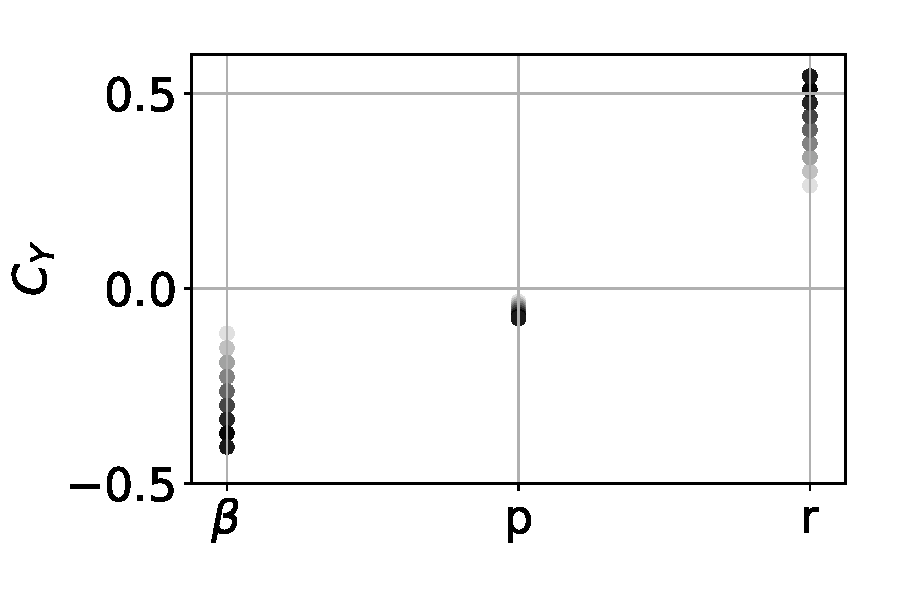
\includegraphics[width=1.0\textwidth]{CyCstAR}
		\caption{All derivatives per rad}
		\label{fig:CyCstAR}
	\end{subfigure}
	%add desired spacing between images, e. g. ~, \quad, \qquad, \hfill etc. 
	%(or a blank line to force the subfigure onto a new line)
	\begin{subfigure}[b]{0.33\textwidth}
		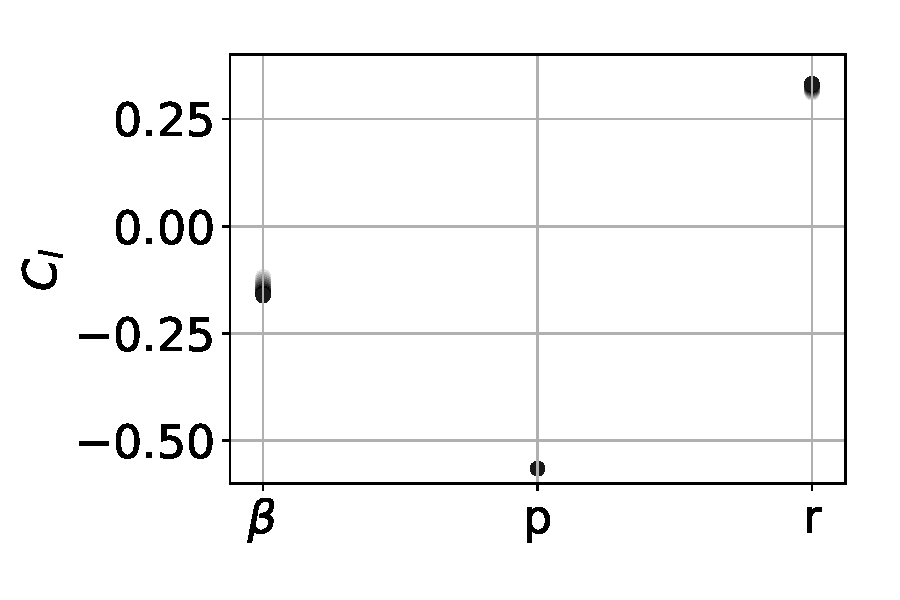
\includegraphics[width=1.0\textwidth]{ClCstAR}
		\caption{All derivatives per rad}
		\label{fig:ClCstAR}
	\end{subfigure}
	%add desired spacing between images, e. g. ~, \quad, \qquad, \hfill etc. 
	%(or a blank line to force the subfigure onto a new line)
	\begin{subfigure}[b]{0.33\textwidth}
		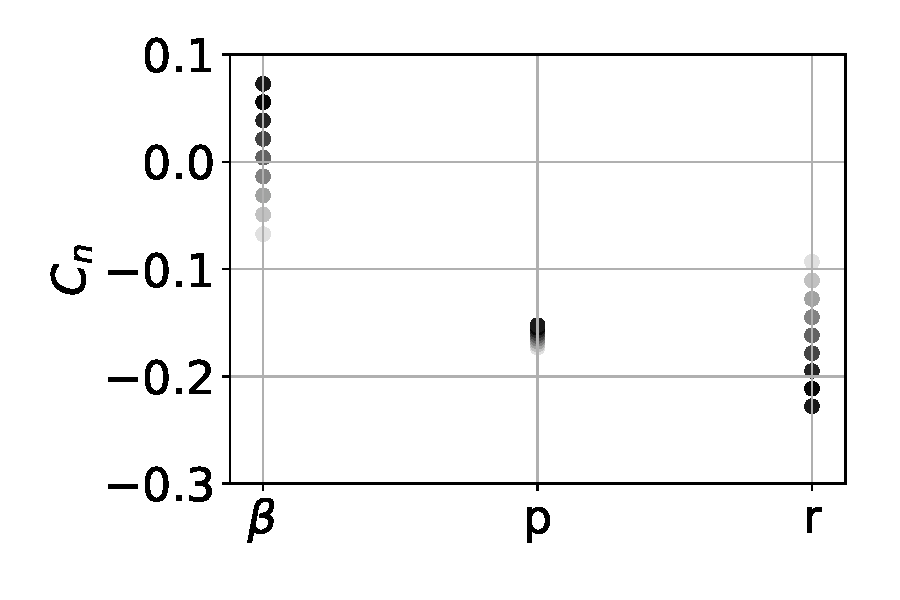
\includegraphics[width=1.0\textwidth]{CnCstAR}
		\caption{All derivatives per rad}
		\label{fig:CnCstAR}
	\end{subfigure}
	\caption{Evolution of lateral coefficients of total aircraft with variation of VT area for constant AR.} Whitest marker represents $S_v=0.1S_{v,0}$, darkest represents $S_v=S_{v,0}$, per step of $0.1S_{v,0}$.\label{fig:cstAR}
\end{figure}

To explore the flight performances in the whole flight envelop, it has been chosen to use a database in function of mach number as only flight parameter. For low speed flight, when the flaps are used, the parameters are assumed to be constant. Then, they vary with the mach number. The evolution of some coefficients with Mach number is illustrated in Fig~\ref{fig:MachVariation}. The Mach number 0.2 taken at see level represents the minimum flight velocity of the ATR72 without flaps.

\begin{figure}[hbt!]
	\centering
	\begin{subfigure}[b]{0.33\textwidth}
		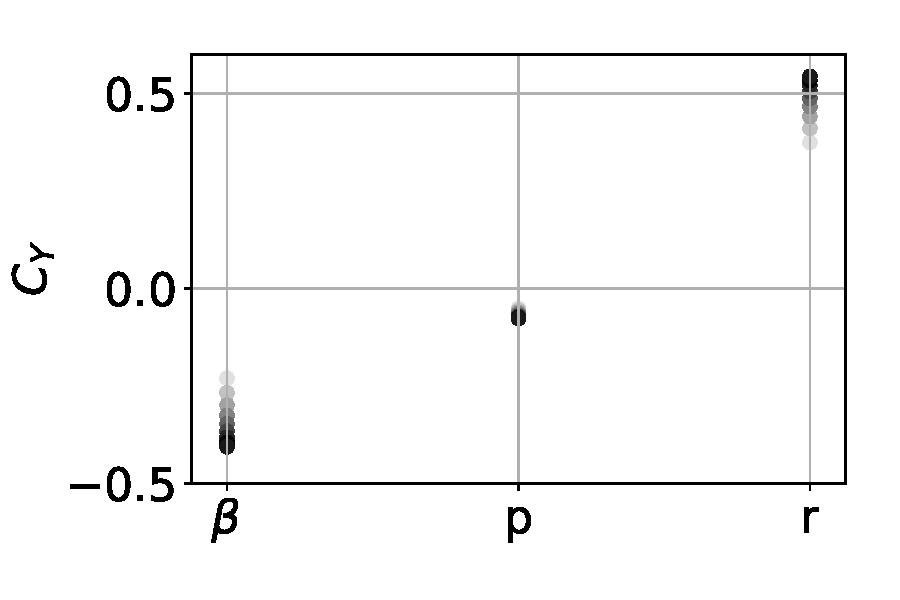
\includegraphics[width=1.0\textwidth]{CyCstSpan}
		\caption{All derivatives per rad}
		\label{fig:CyCstSpan}
	\end{subfigure}
	%add desired spacing between images, e. g. ~, \quad, \qquad, \hfill etc. 
	%(or a blank line to force the subfigure onto a new line)
	\begin{subfigure}[b]{0.33\textwidth}
		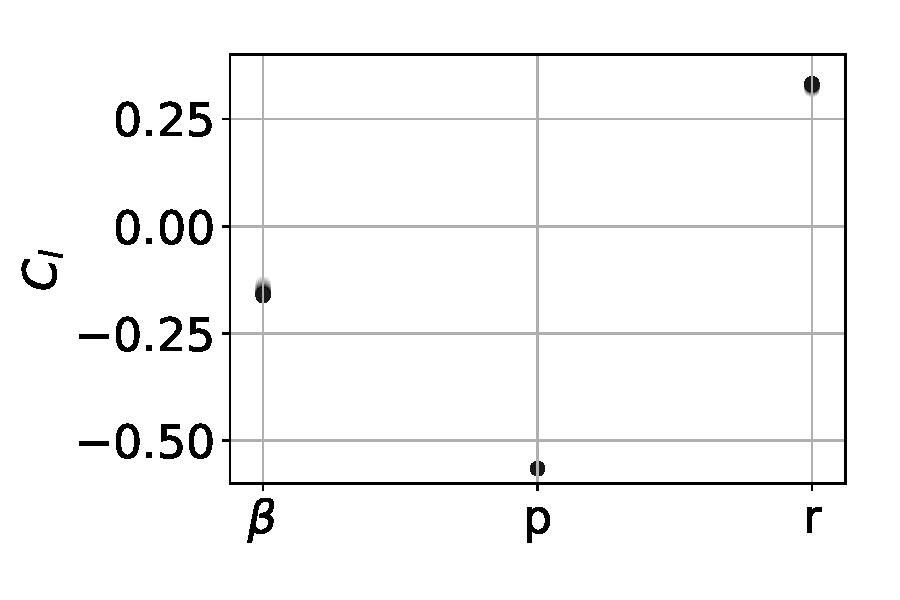
\includegraphics[width=\textwidth]{ClCstSpan}
		\caption{All derivatives per rad}
		\label{fig:ClCstSpan}
	\end{subfigure}
	%add desired spacing between images, e. g. ~, \quad, \qquad, \hfill etc. 
	%(or a blank line to force the subfigure onto a new line)
	\begin{subfigure}[b]{0.33\textwidth}
		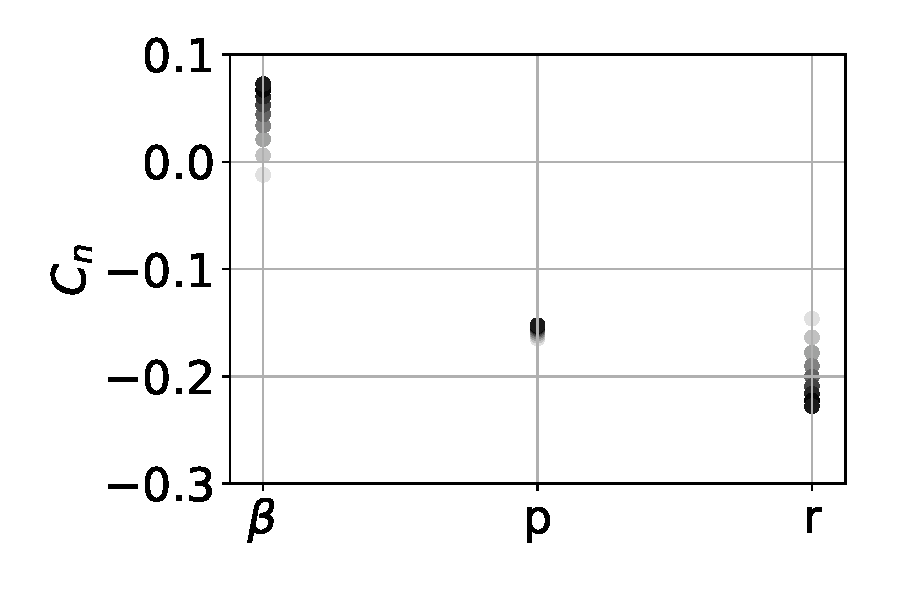
\includegraphics[width=1.0\textwidth]{CnCstSpan}
		\caption{All derivatives per rad}
		\label{fig:CnCstSpan}
	\end{subfigure}
	\caption{Evolution of lateral coefficients of total aircraft with variation of VT area for constant span.} Whitest marker represents $S_v=0.3S_{v,0}$, darkest represents $S_v=S_{v,0}$, per step of $0.1S_{v,0}$ The interval of AR swept is $[1.56,5.21]$\label{fig:cstSpan}
\end{figure}


\begin{figure}[hbt]
	\centering
	\begin{subfigure}[b]{0.49\textwidth}
		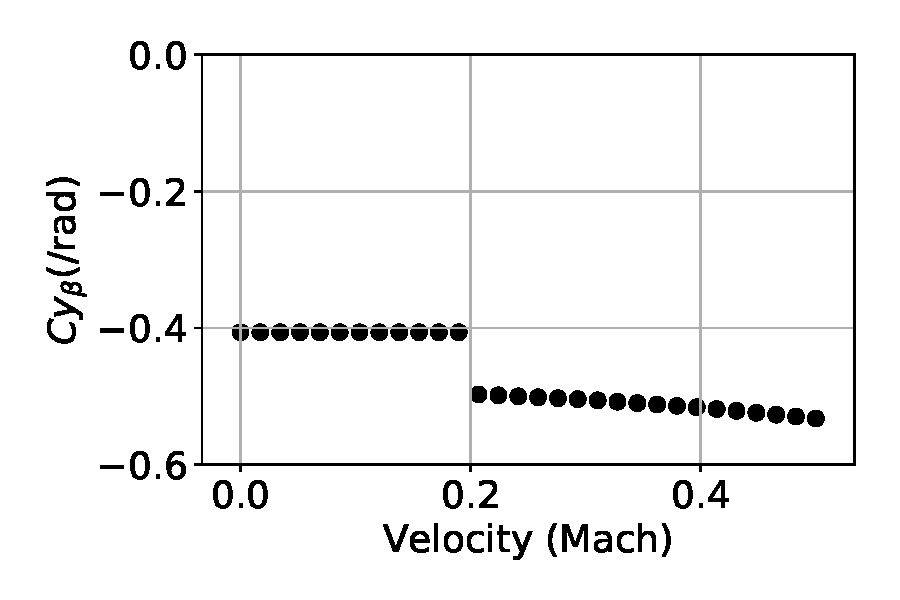
\includegraphics[width=0.8\textwidth]{CybetaMachChange}
		\caption{}
		\label{fig:CybetaMachChange}
	\end{subfigure}
	%add desired spacing between images, e. g. ~, \quad, \qquad, \hfill etc. 
	%(or a blank line to force the subfigure onto a new line)
	\begin{subfigure}[b]{0.49\textwidth}
		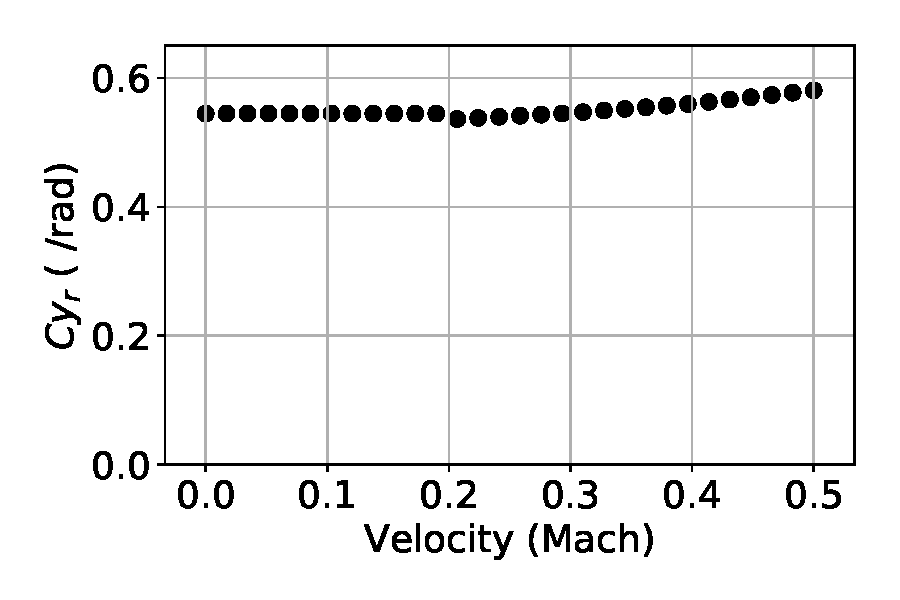
\includegraphics[width=0.8\textwidth]{CyrMachChange}
		\caption{}
		\label{fig:CyrMachChange}
	\end{subfigure}
	\\
	%add desired spacing between images, e. g. ~, \quad, \qquad, \hfill etc. 
	%(or a blank line to force the subfigure onto a new line)
	\begin{subfigure}[b]{0.49\textwidth}
		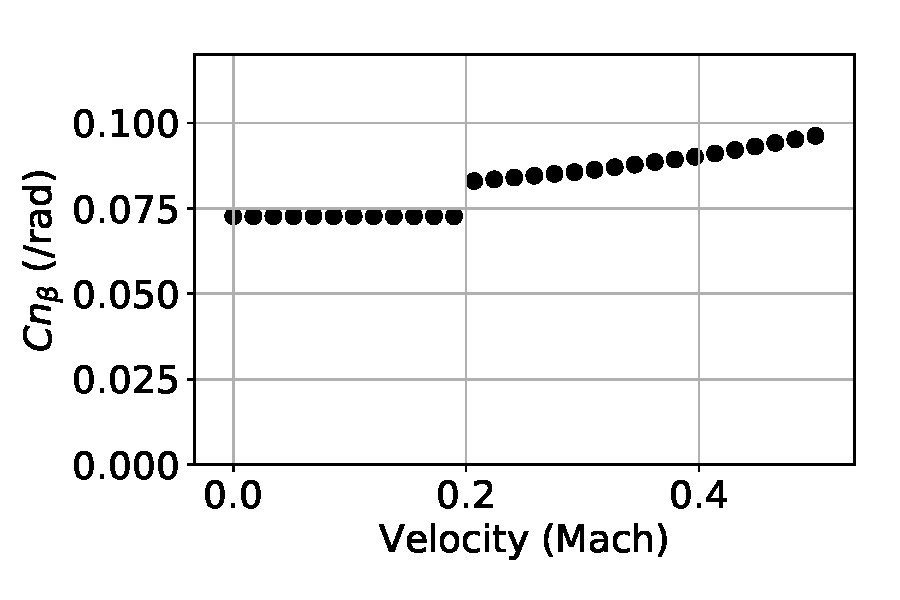
\includegraphics[width=0.8\textwidth]{CnbetaMachChange}
		\caption{}
		\label{fig:CnbetaMachChange}
	\end{subfigure}
	\begin{subfigure}[b]{0.49\textwidth}
		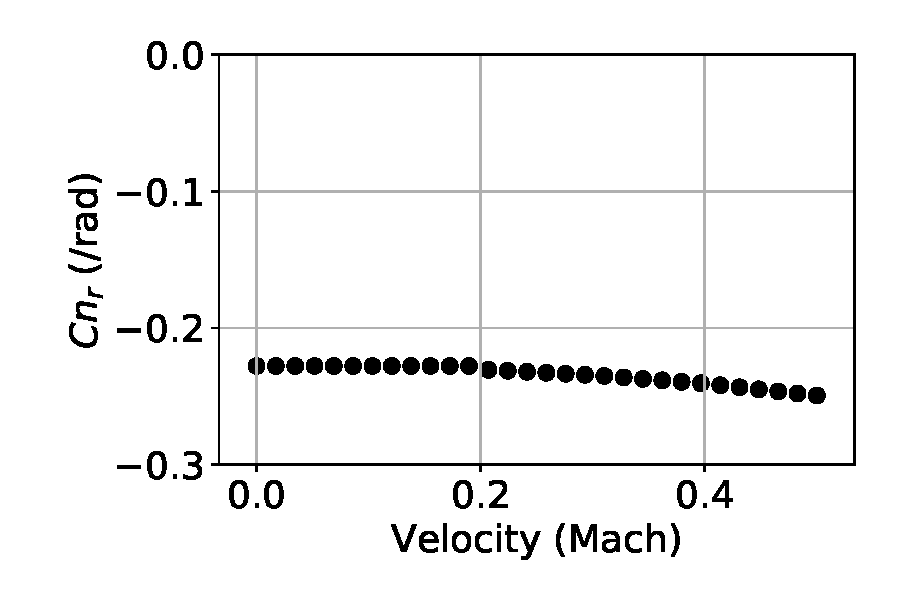
\includegraphics[width=0.8\textwidth]{CnrMachChange}
		\caption{}
		\label{fig:CnrMachChange}
	\end{subfigure}
	\caption{Evolution of lateral coefficients of total aircraft with Mach number.}\label{fig:MachVariation}
\end{figure}

Finally, two ways of modifying the vertical tail are available. The first is the change of surface area while maintaining the aspect ratio constant. This gives linearly varying coefficients as it can be seen in fig~\ref{fig:cstAR}. The second comes from the fact that one may want to keep the horizontal tail high to avoid the slipstream of the propellers, hence the surface should be reduced without modifying the span. In turn the aspect ratio is increased up to reasonnable values to limit extrapolation as shown in fig~\ref{fig:cstSpan}. This variation induces non linear variation of the coefficient and may be find useful for flight qualities.

\begin{table}[hbt]
	\caption{\label{tab:VeDSCParam} A few parameter ranges on which VeDSC has been constructed. From \cite{NicolosiNewApproach}} 
	\centering
	\begin{tabular}{l|l|c}
		Parameters & Description & Range\\
		\hline
		$A_v$ & VT aspect ratio & $\left[1,2\right]$\\
		$A_W$ & Wing aspect ratio & $\left[6,16\right]$\\
		$z_W$ & Wing vertical position, relative to fuselage centerline & $\left[-1,1\right]$ \\
		$z_H$ & Horizontal Tail Vertical Position, relative to VT span & $\left[0,1\right]$\\
		$\frac{S_H}{S_v}$ & Relative Horizontal tail surface area & $\left[0.5,2\right]$
	\end{tabular}
\end{table}